\documentclass[11pt,a4paper]{report}
\usepackage[textwidth=37em,vmargin=30mm]{geometry}
\usepackage{calc,xunicode,amsmath,amssymb,paralist,enumitem,tabu,booktabs,datetime2,xeCJK,xeCJKfntef,listings}
\usepackage{tocloft,fancyhdr,tcolorbox,xcolor,graphicx,eso-pic,xltxtra,xelatexemoji}

\newcommand{\envyear}[0]{2025}
\newcommand{\envdatestr}[0]{2025-08-28}
\newcommand{\envfinaldir}[0]{webdb/2025/20250828/final}

\usepackage[hidelinks]{hyperref}
\hypersetup{
    colorlinks=false,
    pdfpagemode=FullScreen,
    pdftitle={Web Digest - \envdatestr}
}

\setlength{\cftbeforechapskip}{10pt}
\renewcommand{\cftchapfont}{\rmfamily\bfseries\large\raggedright}
\setlength{\cftbeforesecskip}{2pt}
\renewcommand{\cftsecfont}{\sffamily\small\raggedright}

\setdefaultleftmargin{2em}{2em}{1em}{1em}{1em}{1em}

\usepackage{xeCJK,xeCJKfntef}
\xeCJKsetup{PunctStyle=plain,RubberPunctSkip=false,CJKglue=\strut\hskip 0pt plus 0.1em minus 0.05em,CJKecglue=\strut\hskip 0.22em plus 0.2em}
\XeTeXlinebreaklocale "zh"
\XeTeXlinebreakskip = 0pt


\setmainfont{Brygada 1918}
\setromanfont{Brygada 1918}
\setsansfont{IBM Plex Sans}
\setmonofont{JetBrains Mono NL}
\setCJKmainfont{Noto Serif CJK SC}
\setCJKromanfont{Noto Serif CJK SC}
\setCJKsansfont{Noto Sans CJK SC}
\setCJKmonofont{Noto Sans CJK SC}

\setlength{\parindent}{0pt}
\setlength{\parskip}{8pt}
\linespread{1.15}

\lstset{
	basicstyle=\ttfamily\footnotesize,
	numbersep=5pt,
	backgroundcolor=\color{black!5},
	showspaces=false,
	showstringspaces=false,
	showtabs=false,
	tabsize=2,
	captionpos=b,
	breaklines=true,
	breakatwhitespace=true,
	breakautoindent=true,
	linewidth=\textwidth
}






\newcommand{\coverpic}[2]{
    % argv: itemurl, authorname
    Cover photo by #2~~(\href{#1}{#1})
}
\newcommand{\makeheader}[0]{
    \begin{titlepage}
        % \newgeometry{hmargin=15mm,tmargin=21mm,bmargin=12mm}
        \begin{center}
            
            \rmfamily\scshape
            \fontspec{BaskervilleF}
            \fontspec{Old Standard}
            \fontsize{59pt}{70pt}\selectfont
            WEB\hfill DIGEST
            
            \vfill
            % \vskip 30pt
            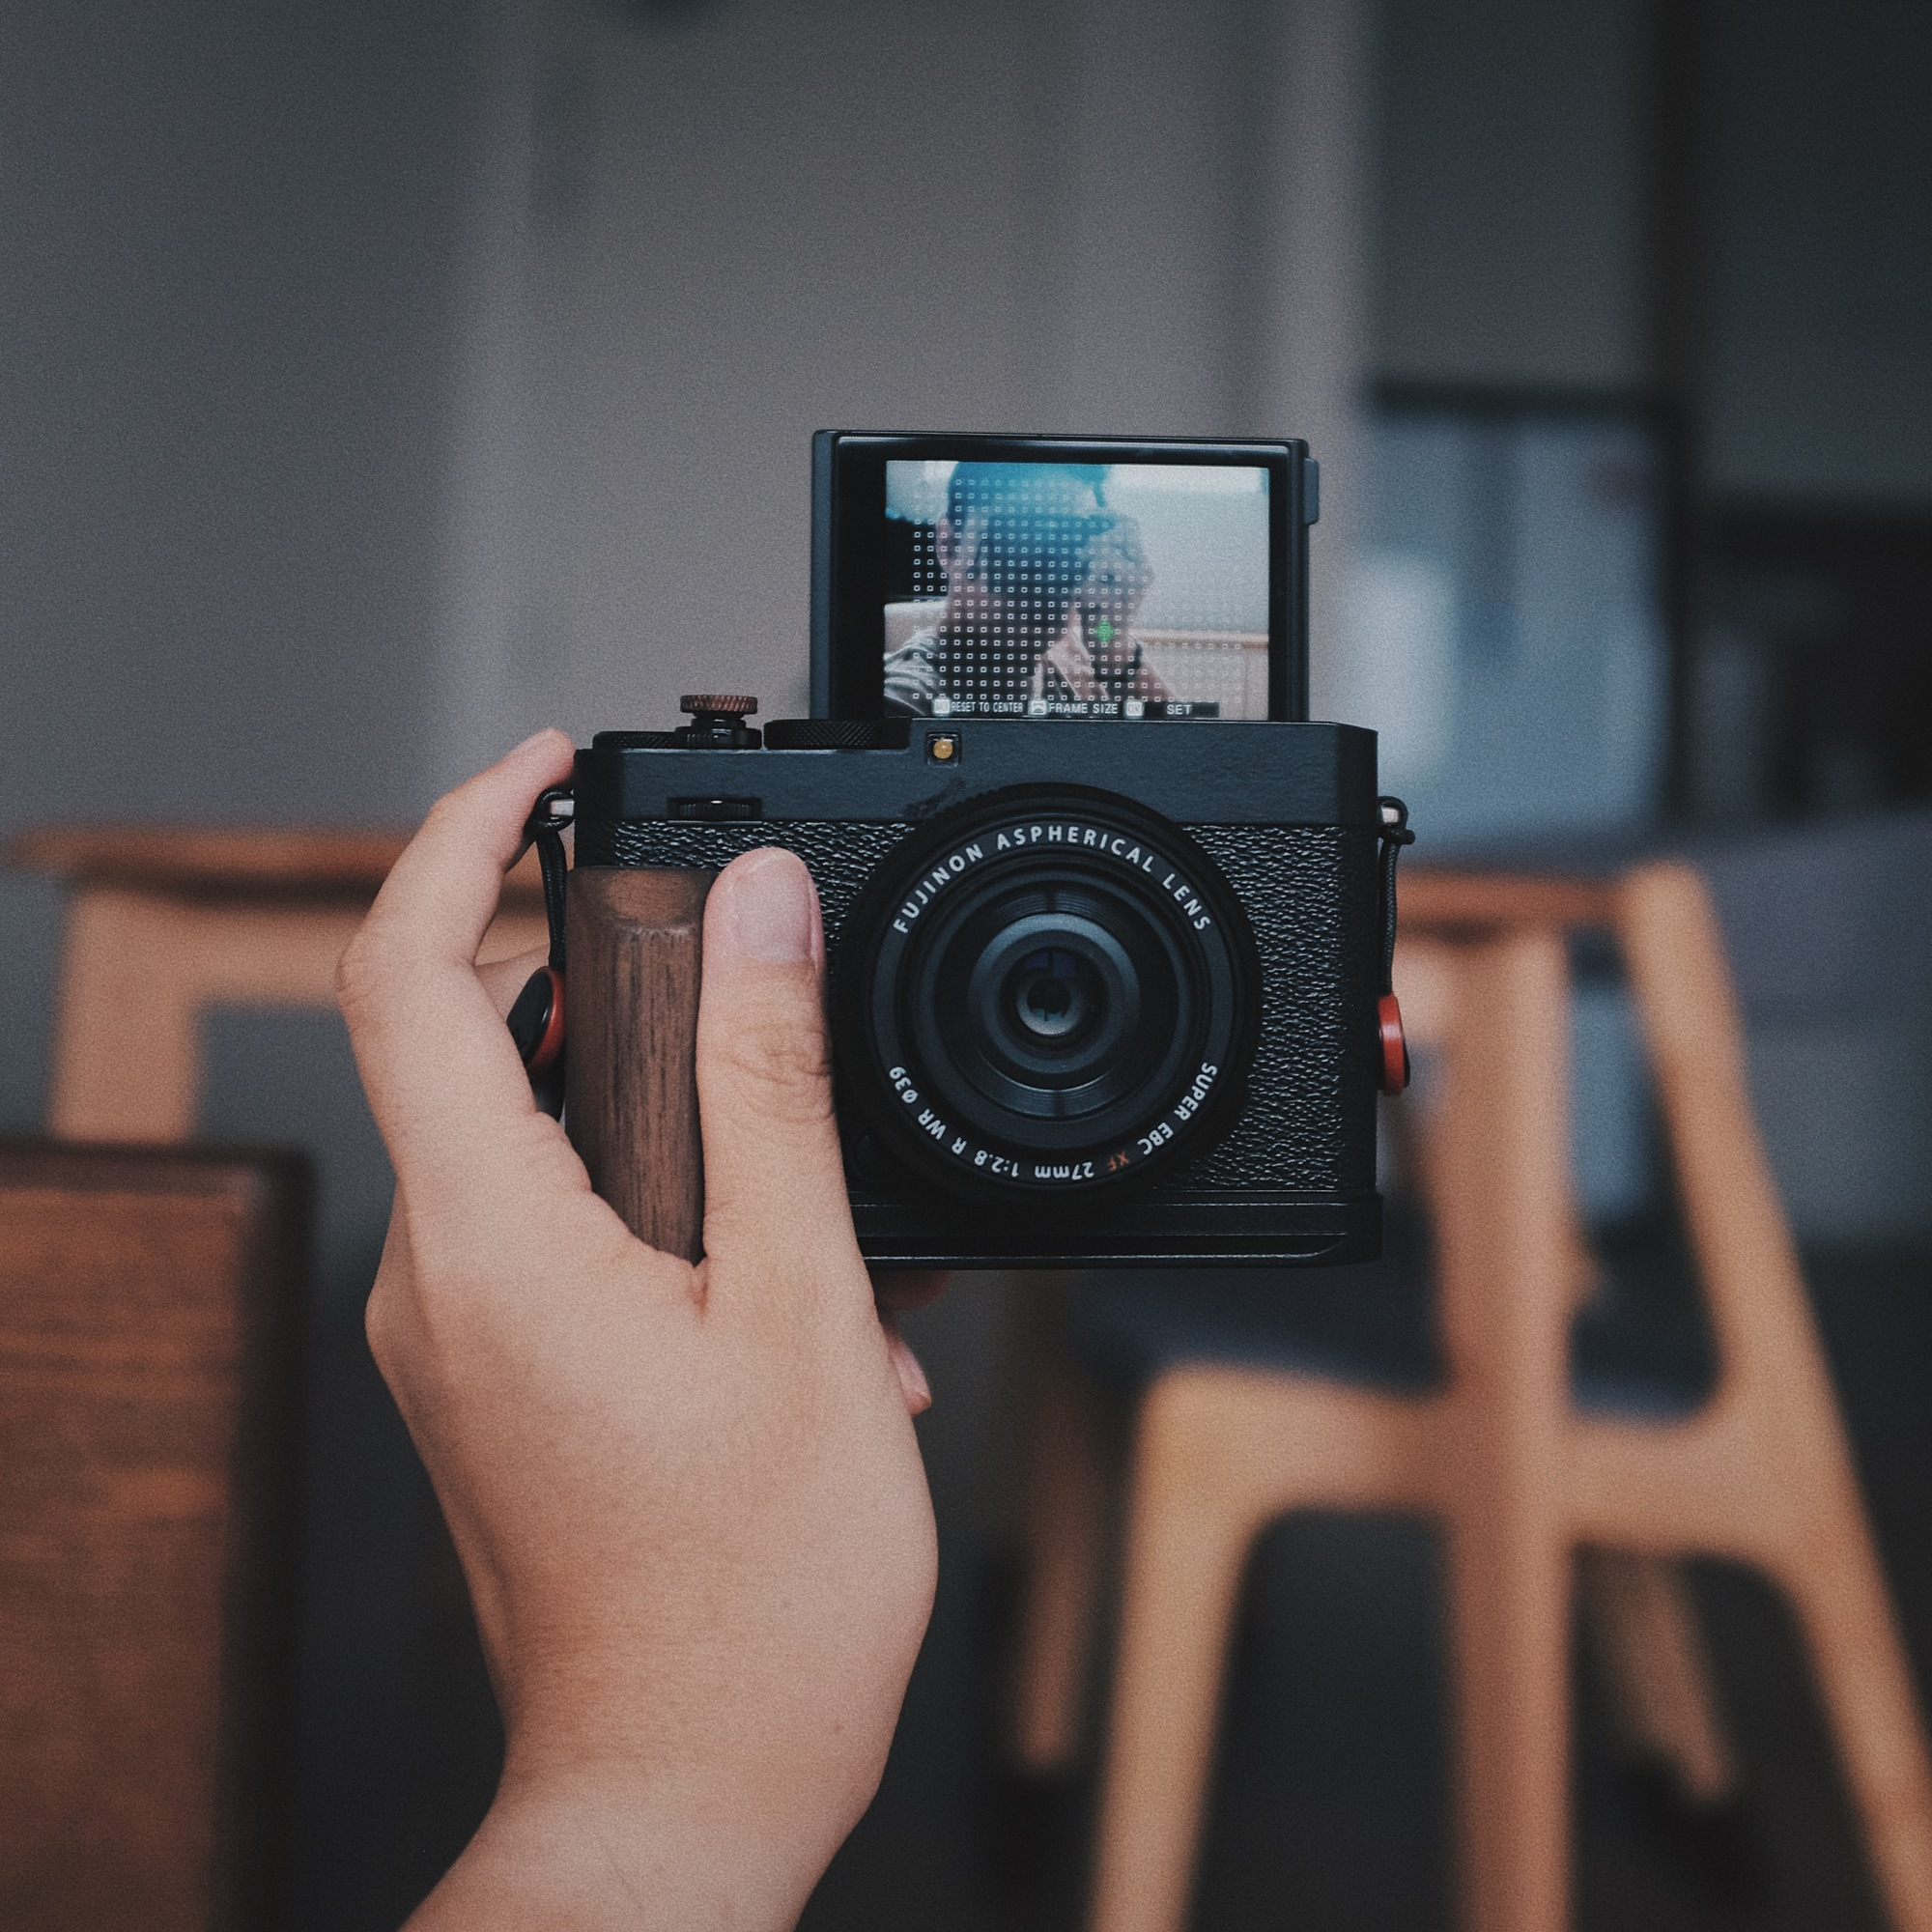
\includegraphics[width=\linewidth]{\envfinaldir/coverpic-prod.jpg}\par
            % \vskip 30pt
            \vfill

            \normalsize\rmfamily\scshape
            \copyright{} The Web Digest Project \hfill\large \envdatestr
        \end{center}
    \end{titlepage}
    % \restoregeometry
}
\newcommand{\simplehref}[1]{%
    \textcolor{blue!80!green}{\href{#1}{#1}}%
}
\renewcommand{\contentsname}{\center\Huge\sffamily\bfseries Contents\par\vskip 20pt}
\newcounter{ipartcounter}
\setcounter{ipartcounter}{0}
\newcommand{\ipart}[1]{
    % \vskip 20pt
    \clearpage
    \stepcounter{ipartcounter}
    \phantomsection
    \addcontentsline{toc}{chapter}{#1}
    % \begin{center}
    %     \Huge
    %     \sffamily\bfseries
    %     #1
    % \end{center}
    % \vskip 20pt plus 7pt
}
\newcounter{ichaptercounter}
\setcounter{ichaptercounter}{0}
\newcommand{\ichapter}[1]{
    % \vskip 20pt
    \clearpage
    \stepcounter{ichaptercounter}
    \phantomsection
    \addcontentsline{toc}{section}{\numberline{\arabic{ichaptercounter}}#1}
    \begin{center}
        \Huge
        \sffamily\bfseries
        #1
    \end{center}
    \vskip 20pt plus 7pt
}
\newcommand{\entrytitlefont}[1]{\subsection*{\raggedright\Large\sffamily\bfseries#1}}
\newcommand{\entryitemGeneric}[2]{
    % argv: title, url
    \parbox{\linewidth}{
        \entrytitlefont{#1}\par\vskip 5pt
        \footnotesize\ttfamily\mdseries
        \simplehref{#2}
    }\vskip 11pt plus 11pt minus 1pt
}
\newcommand{\entryitemGithub}[3]{
    % argv: title, url, desc
    \parbox{\linewidth}{
        \entrytitlefont{#1}\par\vskip 5pt
        \footnotesize\ttfamily\mdseries
        \simplehref{#2}\par\vskip 5pt
        \small\rmfamily\mdseries#3
    }\vskip 11pt plus 11pt minus 1pt
}
\newcommand{\entryitemAp}[3]{
    % argv: title, url, desc
    \parbox{\linewidth}{
        \entrytitlefont{#1}\par\vskip 5pt
        \footnotesize\ttfamily\mdseries
        \simplehref{#2}\par\vskip 5pt
        \small\rmfamily\mdseries#3
    }\vskip 11pt plus 11pt minus 1pt
}
\newcommand{\entryitemHackernews}[3]{
    % argv: title, hnurl, rawurl
    % \parbox{\linewidth}{
    %     \entrytitlefont{#1}\par\vskip 5pt
    %     \footnotesize\ttfamily\mdseries
    %     \simplehref{#3}\par
    %     \textcolor{black!50}{\href{#2}{#2}}
    % }\vskip 11pt plus 11pt minus 1pt
    \begin{minipage}{\linewidth}
            \entrytitlefont{#1}\par\vskip 5pt
            \footnotesize\ttfamily\mdseries
            \simplehref{#3}\par
            \textcolor{black!50}{\href{#2}{#2}}
    \end{minipage}\par\vskip 11pt plus 11pt minus 1pt
}







\begin{document}

\makeheader

\tableofcontents\clearpage




\ipart{Developers}
\ichapter{Hacker News}
\entryitemTwoLinks{Google has eliminated 35\% of managers overseeing small teams in past year}{https://news.ycombinator.com/item?id=45045398}{https://www.cnbc.com/2025/08/27/google-executive-says-company-has-cut-a-third-of-its-managers.html}

\entryitemTwoLinks{Beginning 1 September, we will need to geoblock Mississippi IPs}{https://news.ycombinator.com/item?id=45044440}{https://dw-news.dreamwidth.org/44429.html}

\entryitemTwoLinks{Mapping connections of anti-offshore wind groups and their lawyers}{https://news.ycombinator.com/item?id=45044168}{https://www.climatedevlab.brown.edu/post/legal-entanglements-mapping-connections-of-anti-offshore-wind-groups-and-their-lawyers-in-the-easte}

\entryitemTwoLinks{I Am An AI Hater}{https://news.ycombinator.com/item?id=45043741}{https://anthonymoser.github.io/writing/ai/haterdom/2025/08/26/i-am-an-ai-hater.html}

\entryitemTwoLinks{Firefox Has Moved to Firefox.com}{https://news.ycombinator.com/item?id=45043545}{https://www.firefox.com}

\entryitemTwoLinks{House to investigate Wikipedia over allegations of organized bias}{https://news.ycombinator.com/item?id=45043164}{https://thehill.com/homenews/house/5473331-wikipedia-bias-probe-republicans/}

\entryitemTwoLinks{A failure of security systems at PayPal is causing concern for German banks}{https://news.ycombinator.com/item?id=45042461}{https://www.nordbayern.de/news-in-english/paypal-security-systems-down-german-banks-block-payments-in-the-billions-1.14811187}

\entryitemTwoLinks{Typepad is shutting down}{https://news.ycombinator.com/item?id=45041807}{https://everything.typepad.com/blog/2025/08/typepad-is-shutting-down.html}

\entryitemTwoLinks{GMP damaging Zen 5 CPUs?}{https://news.ycombinator.com/item?id=45041743}{https://gmplib.org/gmp-zen5}

\entryitemTwoLinks{VIM Master}{https://news.ycombinator.com/item?id=45041315}{https://github.com/renzorlive/vimmaster}

\entryitemTwoLinks{Unexpected productivity boost of Rust}{https://news.ycombinator.com/item?id=45041286}{https://lubeno.dev/blog/rusts-productivity-curve}

\entryitemTwoLinks{Launch HN: Bitrig (YC S25) – Build Swift apps on your iPhone}{https://news.ycombinator.com/item?id=45041185}{https://news.ycombinator.com/item?id=45041185}

\entryitemTwoLinks{Apple revokes EU distribution rights for an app on the Alt Store}{https://news.ycombinator.com/item?id=45040064}{https://torrentfreak.com/apple-revokes-eu-distribution-rights-for-torrent-client-developer-left-in-the-dark/}

\entryitemTwoLinks{Implementing Forth in Go and C}{https://news.ycombinator.com/item?id=45039301}{https://eli.thegreenplace.net/2025/implementing-forth-in-go-and-c/}

\entryitemTwoLinks{SpaceX's giant Starship Mars rocket nails critical 10th test flight}{https://news.ycombinator.com/item?id=45039075}{https://www.space.com/space-exploration/private-spaceflight/spacex-launches-starship-flight-10-critical-test-flight-video}

\entryitemTwoLinks{Bring Your Own Agent to Zed – Featuring Gemini CLI}{https://news.ycombinator.com/item?id=45038710}{https://zed.dev/blog/bring-your-own-agent-to-zed}

\entryitemTwoLinks{Nx compromised: malware uses Claude code CLI to explore the filesystem}{https://news.ycombinator.com/item?id=45038653}{https://semgrep.dev/blog/2025/security-alert-nx-compromised-to-steal-wallets-and-credentials/}

\entryitemTwoLinks{ASCIIFlow}{https://news.ycombinator.com/item?id=45038565}{https://asciiflow.com/}

\entryitemTwoLinks{F-35 pilot held 50-minute airborne conference call with engineers before crash}{https://news.ycombinator.com/item?id=45038261}{https://www.cnn.com/2025/08/27/us/alaska-f-35-crash-accident-report-hnk-ml}

\entryitemTwoLinks{How to slow down a program and why it can be useful}{https://news.ycombinator.com/item?id=45038260}{https://stefan-marr.de/2025/08/how-to-slow-down-a-program/}


\ipart{Developers~~~~(zh-Hans)}
\ichapter{Solidot}
\entryitemGeneric{\hskip 0pt{}Google 在翻译应用中加入 AI 驱动的语言学习功能}{https://www.solidot.org/story?sid=82151}

\entryitemGeneric{\hskip 0pt{}父母指控 OpenAI 的 ChatGPT 杀死了他们的孩子}{https://www.solidot.org/story?sid=82150}

\entryitemGeneric{\hskip 0pt{}苹果讨论过收购 Mistral AI 和 Perplexity}{https://www.solidot.org/story?sid=82149}

\entryitemGeneric{\hskip 0pt{}Anthropic 与图书作者就侵犯版权达成和解}{https://www.solidot.org/story?sid=82148}

\entryitemGeneric{\hskip 0pt{}无印良品在华商标诉讼败诉}{https://www.solidot.org/story?sid=82147}

\entryitemGeneric{\hskip 0pt{}马斯克的 xAI 起诉苹果和 OpenAI 阻碍竞争}{https://www.solidot.org/story?sid=82146}

\entryitemGeneric{\hskip 0pt{}暴露在热浪下会加速衰老}{https://www.solidot.org/story?sid=82145}

\entryitemGeneric{\hskip 0pt{}英特尔警告美国政府控股可能引发负面反应}{https://www.solidot.org/story?sid=82144}

\entryitemGeneric{\hskip 0pt{}苹果指控前雇员为 Oppo 窃取智能手表的商业机密}{https://www.solidot.org/story?sid=82143}

\entryitemGeneric{\hskip 0pt{}Google 将从明年屏蔽未验证开发者的 Android 应用的侧载}{https://www.solidot.org/story?sid=82142}

\entryitemGeneric{\hskip 0pt{}Twitch 打击机器人账号,部分频道的观看者减少了一半}{https://www.solidot.org/story?sid=82141}

\entryitemGeneric{\hskip 0pt{}X-37B 将测试量子惯性传感器}{https://www.solidot.org/story?sid=82140}

\entryitemGeneric{\hskip 0pt{}研究发现长时间接触食物气味会抑制食物摄入}{https://www.solidot.org/story?sid=82139}

\entryitemGeneric{\hskip 0pt{}高温美发过程可能释放逾百亿纳米颗粒}{https://www.solidot.org/story?sid=82138}

\entryitemGeneric{\hskip 0pt{}英伟达探索 H20 后续产品}{https://www.solidot.org/story?sid=82137}

\entryitemGeneric{\hskip 0pt{}Bluesky 屏蔽密西西比州用户访问其服务}{https://www.solidot.org/story?sid=82136}

\entryitemGeneric{\hskip 0pt{}谷神星可能曾经宜居}{https://www.solidot.org/story?sid=82135}

\entryitemGeneric{\hskip 0pt{}小肯尼迪要求撤回一篇疫苗研究论文,期刊拒绝}{https://www.solidot.org/story?sid=82134}\ichapter{V2EX}
\entryitemGeneric{\hskip 0pt{}[职场话题] 求助 DevOps | Infra 同行}{https://www.v2ex.com/t/1155406}

\entryitemGeneric{\hskip 0pt{}[问与答] 集思广益, AI 及各种机器人发展能让哪些行业利润率暴增呢}{https://www.v2ex.com/t/1155405}

\entryitemGeneric{\hskip 0pt{}[macOS] 2020 款 15 寸体验 Tahoe 26 系统}{https://www.v2ex.com/t/1155402}

\entryitemGeneric{\hskip 0pt{}[户外运动] 单日徒步有什么性价比运动手表推荐吗}{https://www.v2ex.com/t/1155400}

\entryitemGeneric{\hskip 0pt{}[程序员] 让 AI 搓网页太丑!如何培养自己的审美?或者让 AI 先产出设计再产出页面?}{https://www.v2ex.com/t/1155399}

\entryitemGeneric{\hskip 0pt{}[宽带症候群] 广电这种老光猫可以抓直播源吗}{https://www.v2ex.com/t/1155396}

\entryitemGeneric{\hskip 0pt{}[分享创造] 2 周搓了个 web 界面,多人群聊,自定义开场白结束语,这个播客生成器邀请 V2ER 试用}{https://www.v2ex.com/t/1155395}

\entryitemGeneric{\hskip 0pt{}[Apple] 美区购买的 infuse,国区账号如何恢复?}{https://www.v2ex.com/t/1155394}

\entryitemGeneric{\hskip 0pt{}[YouTube] Youtube 的自动音轨翻译功能就是反人类}{https://www.v2ex.com/t/1155393}

\entryitemGeneric{\hskip 0pt{}[奇思妙想] 智能眼镜应用遐思}{https://www.v2ex.com/t/1155391}

\entryitemGeneric{\hskip 0pt{}[生活] 请教一下大家是怎么管教自己孩子看电视看手机的问题的?}{https://www.v2ex.com/t/1155390}

\entryitemGeneric{\hskip 0pt{}[加密货币] 最近几天的炒币情况}{https://www.v2ex.com/t/1155388}

\entryitemGeneric{\hskip 0pt{}[Next.js] 分享 Next.js 15.2 之后新版本的一个坑,可能会影响你的 SEO 收录}{https://www.v2ex.com/t/1155386}

\entryitemGeneric{\hskip 0pt{}[问与答] 9 月 1 号新规之后 必要缴纳社保, 同时持有保安之类的 城市社保 和 农村社保 , 怎么处理能够利益最大化?}{https://www.v2ex.com/t/1155385}

\entryitemGeneric{\hskip 0pt{}[计算机] 为什么感觉现在组一台电脑和一年前的价格差不多?}{https://www.v2ex.com/t/1155384}

\entryitemGeneric{\hskip 0pt{}[汽车] 哪些汽车出厂自带的功能,是你几乎没用过的?}{https://www.v2ex.com/t/1155383}

\entryitemGeneric{\hskip 0pt{}[问与答] 安卓系统学英语软件突然不发声的奇怪问题求助}{https://www.v2ex.com/t/1155382}

\entryitemGeneric{\hskip 0pt{}[分享发现] AI 编程真是太好用了,分分钟钟搞定 一个 Minecraft 圆形生成器}{https://www.v2ex.com/t/1155380}

\entryitemGeneric{\hskip 0pt{}[生活] 买房抉择 绍兴还是义乌?}{https://www.v2ex.com/t/1155379}

\entryitemGeneric{\hskip 0pt{}[分享发现] 如何看待钉钉 CEO 无招:四五十人拼 DingTalk A1 四个月,每天睡眠不足 5 小时}{https://www.v2ex.com/t/1155377}

\entryitemGeneric{\hskip 0pt{}[职场话题] 如今行情到底如何?大龄想出来看工作了}{https://www.v2ex.com/t/1155376}

\entryitemGeneric{\hskip 0pt{}[奇思妙想] 在 2048 小游戏基础上 开发了一个 2048 小蛋糕游戏}{https://www.v2ex.com/t/1155375}

\entryitemGeneric{\hskip 0pt{}[Arc] 我被 arc 浏览器拉黑了?}{https://www.v2ex.com/t/1155374}

\entryitemGeneric{\hskip 0pt{}[程序员] 目前在 jetbrains 全家桶里面最好用的自动完成插件是哪个?}{https://www.v2ex.com/t/1155372}

\entryitemGeneric{\hskip 0pt{}[职场话题] 第一次遇到听不懂人话的 HR}{https://www.v2ex.com/t/1155371}

\entryitemGeneric{\hskip 0pt{}[分享创造] Chrome 离线翻译插件 版本大更新!}{https://www.v2ex.com/t/1155370}

\entryitemGeneric{\hskip 0pt{}[Linux] 请教下 ubuntu18 下 双网卡配置, netplan 配置会不生效的问题}{https://www.v2ex.com/t/1155368}

\entryitemGeneric{\hskip 0pt{}[酷工作] [广州-三七互娱-社招] Golang 开发工程师}{https://www.v2ex.com/t/1155367}

\entryitemGeneric{\hskip 0pt{}[问与答] 有什么轻便 1w 毫安 [充电宝] 可以推荐吗?}{https://www.v2ex.com/t/1155365}

\entryitemGeneric{\hskip 0pt{}[宽带症候群] 佛山顺德 电信公网 IP 问题}{https://www.v2ex.com/t/1155364}

\entryitemGeneric{\hskip 0pt{}[问与答] sedo 售出域名后,选择电汇到国内,一般需要多久呢?}{https://www.v2ex.com/t/1155363}

\entryitemGeneric{\hskip 0pt{}[程序员] Hulo 语言开发分享 —— 调试器是如何工作的?}{https://www.v2ex.com/t/1155362}

\entryitemGeneric{\hskip 0pt{}[Apple TV] 115 生活上架 App Store,支持 Apple TV。}{https://www.v2ex.com/t/1155361}

\entryitemGeneric{\hskip 0pt{}[问与答] 我该何去何从?}{https://www.v2ex.com/t/1155359}

\entryitemGeneric{\hskip 0pt{}[问与答] 广电的流量卡在深圳体验如何}{https://www.v2ex.com/t/1155358}

\entryitemGeneric{\hskip 0pt{}[职场话题] 梦网科技}{https://www.v2ex.com/t/1155357}

\entryitemGeneric{\hskip 0pt{}[生活] 真的好无聊}{https://www.v2ex.com/t/1155356}

\entryitemGeneric{\hskip 0pt{}[Android] 安卓手机录屏录音方案求推荐}{https://www.v2ex.com/t/1155355}

\entryitemGeneric{\hskip 0pt{}[Google] 突然 Google AI Studio 不能用了,悲伤😭😭😭}{https://www.v2ex.com/t/1155354}

\entryitemGeneric{\hskip 0pt{}[分享发现] 开发一个最近很火的手办生成器,目前免费欢迎使用}{https://www.v2ex.com/t/1155353}

\entryitemGeneric{\hskip 0pt{}[Solana] 这个大佬是定投了吧, 还是怕一次性买入把价格拉上去.}{https://www.v2ex.com/t/1155352}

\entryitemGeneric{\hskip 0pt{}[Cursor] cursor 编程经验分享}{https://www.v2ex.com/t/1155350}

\entryitemGeneric{\hskip 0pt{}[投资] 大 a 今天开始``技术性调整'',信长牛大牛的可以一股脑梭进去了}{https://www.v2ex.com/t/1155348}

\entryitemGeneric{\hskip 0pt{}[推广] 你们尝试 Nano Banana 模型了吗?}{https://www.v2ex.com/t/1155347}

\entryitemGeneric{\hskip 0pt{}[iPhone] 你的 Action 按键设置的是什么动作?}{https://www.v2ex.com/t/1155346}

\entryitemGeneric{\hskip 0pt{}[Solana] 美股代币化:金融创新、市场博弈与监管重构}{https://www.v2ex.com/t/1155345}

\entryitemGeneric{\hskip 0pt{}[分享发现] 八部金刚功治好了空调吹出的肩颈疼痛}{https://www.v2ex.com/t/1155343}

\entryitemGeneric{\hskip 0pt{}[问与答] 十万火急 家人意外去世 华为 mate60 能否在保数据的情况下解锁?}{https://www.v2ex.com/t/1155342}

\entryitemGeneric{\hskip 0pt{}[Solana] V2EX 联动 OKX 欧易!限时 30 天—— 新人最高获 151.66U,老用户交易得 20U}{https://www.v2ex.com/t/1155341}

\entryitemGeneric{\hskip 0pt{}[问与答] 第一次写 springboot 项目,不知道如何进行压力测试,用满服务器资源,求大佬执教}{https://www.v2ex.com/t/1155340}


\ipart{Generic News}







\clearpage
\leavevmode\vfill
\footnotesize

Copyright \copyright{} 2023-2025 Neruthes and other contributors.

This document is published with CC BY-NC-ND 4.0 license.

The entries listed in this newsletter may be copyrighted by their respective creators.

This newsletter is generated by the Web Digest project.

The newsletters are also delivered via Telegram channel \CJKunderline{\href{https://t.me/webdigestchannel}{https://t.me/webdigestchannel}}.\\
RSS feed is available at \CJKunderline{\href{https://webdigest.pages.dev/rss.xml}{https://webdigest.pages.dev/rss.xml}}.

This newsletter is available in PDF at
\CJKunderline{\href{https://webdigest.pages.dev/}{https://webdigest.pages.dev/}}.

The source code being used to generate this newsletter is available at\\
\CJKunderline{\href{https://github.com/neruthes/webdigest}{https://github.com/neruthes/webdigest}}.

This newsletter is also available in
\CJKunderline{\href{http://webdigest.pages.dev/readhtml/\envyear/WebDigest-20250828.html}{HTML}} and
\CJKunderline{\href{https://github.com/neruthes/webdigest/blob/master/markdown/\envyear/WebDigest-20250828.md}{Markdown}}.


\coverpic{https://unsplash.com/photos/a-snowy-lake-with-a-small-boathouse-8Z-4GMhsics}{Hunter Reilly}


\end{document}
